\documentclass[a4paper,11pt]{article}%
\usepackage{a4wide}%

\usepackage[english]{babel}%
\usepackage[utf8]{inputenc}%
\usepackage[T1]{fontenc}%

\usepackage{caption}
\usepackage{subcaption}

\usepackage{graphicx}%
\usepackage{xspace}%

\usepackage{url} \urlstyle{sf}%
\DeclareUrlCommand\email{\urlstyle{sf}}%

\usepackage{mathpazo}%
\let\bfseriesaux=\bfseries%
\renewcommand{\bfseries}{\sffamily\bfseriesaux}

\newenvironment{keywords}%
{\description\item[Keyword.]}%
{\enddescription}


\newenvironment{remarque}%
{\description\item[Remark.]\sl}%
{\enddescription}

\font\manual=manfnt
\newcommand{\dbend}{{\manual\char127}}

\newenvironment{attention}%
{\description\item[\dbend]\sl}%
{\enddescription}

\usepackage{listings}%

\lstset{%
  basicstyle=\sffamily,%
  columns=fullflexible,%
  language=caml,%
  frame=lb,%
  frameround=fftf,%
}%

\lstMakeShortInline{|}

\parskip=0.3\baselineskip%
\sloppy%


\usepackage{float}  % H option for figures

%%%%%%%%%%%%%%%%%%%%%%%%%%%%%%%%%%%%%%%%%%%%%%%%%

\begin{document}

\title{Delaunay's triangulation \\ Project 2 PROG1}

\author{Simon Bihel}

\date{November 8, 2015}

\maketitle

\begin{abstract}
	This report will present and discuss my work on the second project of the course PROG1.
\begin{keywords}
	Delaunay; triangulation; convex hull.
\end{keywords}
\end{abstract}


\section{Basic program}

The obligatory part of the project was well guided and so I will talk about the approach I took to do the various functions. The result is shown in the figure~\ref{fig:basic} 

\begin{figure}[H]
	\begin{center}
		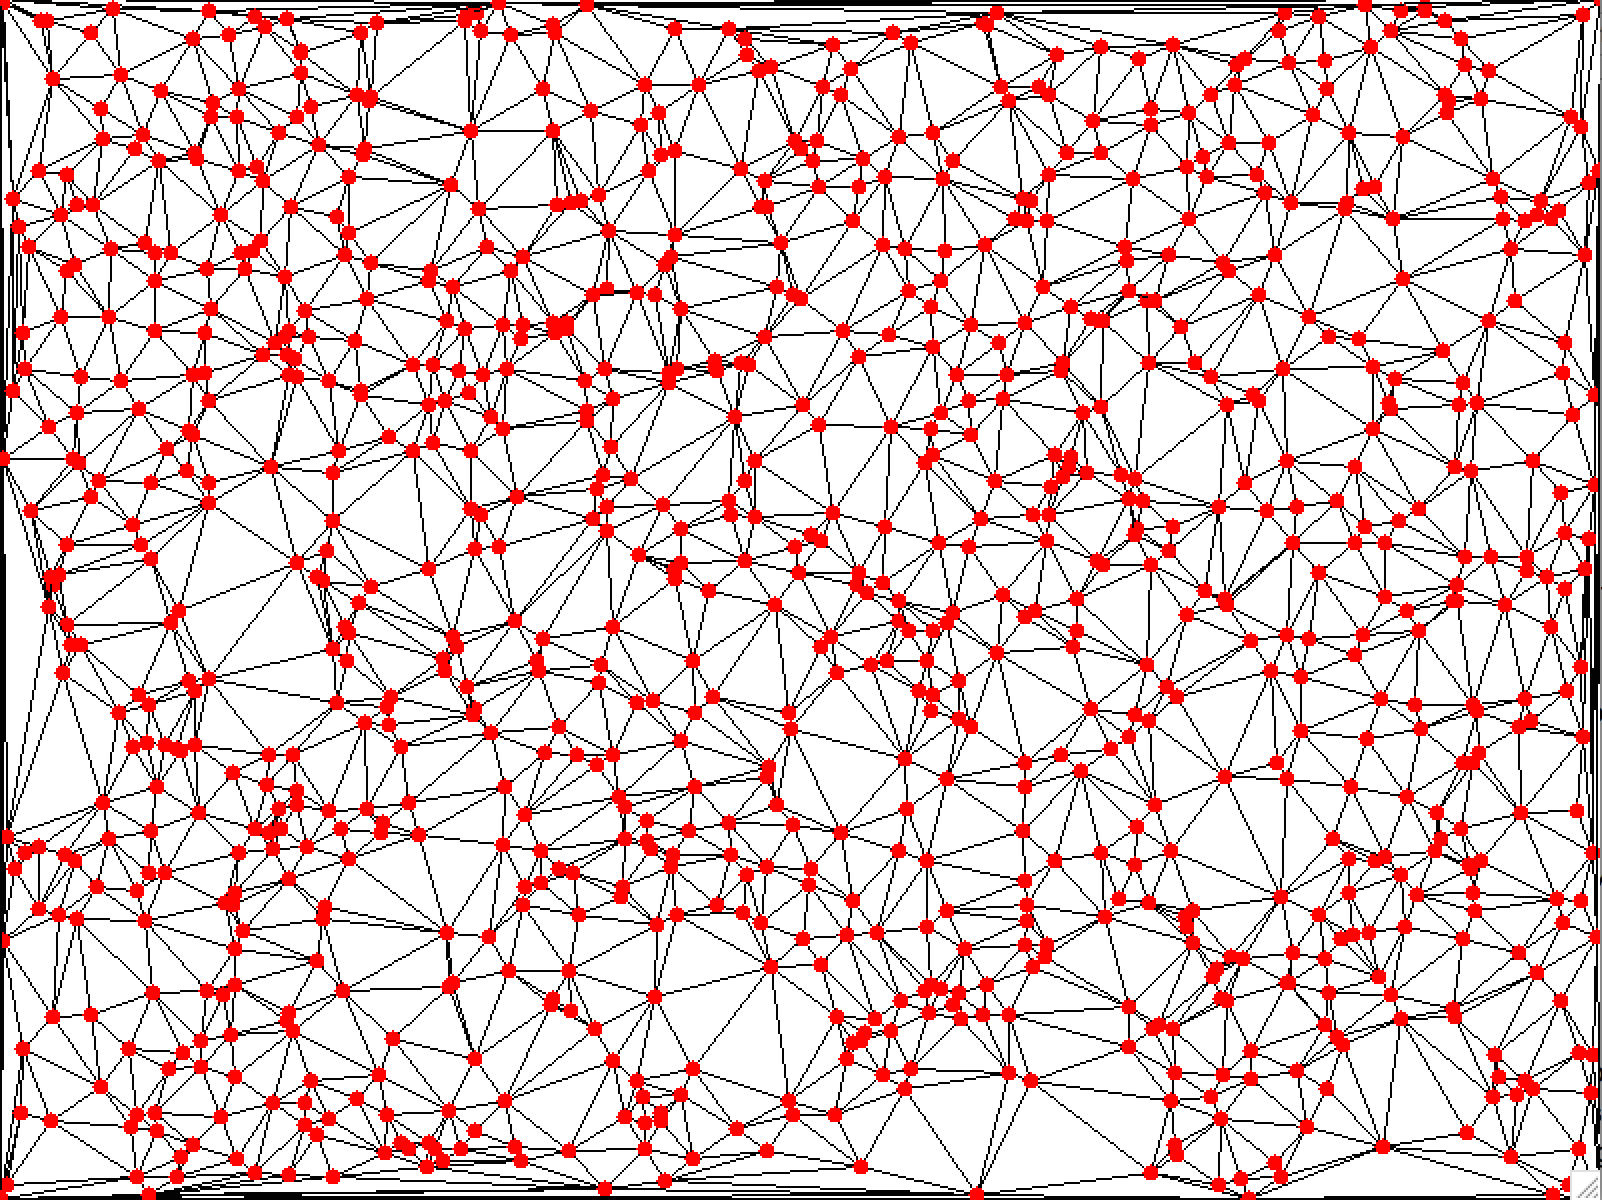
\includegraphics[scale=0.3]{basic.png}
	\end{center}
	\caption{Basic version of the Delaunay's triangulation}
	\label{fig:basic}
\end{figure}

I decided to do simple functions, like for |border| where I simply get all the edges and then keep the single ones going twice through the list. The complexity isn't the best but it is quite clear of what the function does. \\


With the basic version covered, we can now talk about the extensions.



\section{Advanced program}

The main extension that I decided to add was the triangulation without adding points, thus starting with the convex hull of the existing points. The result is shown in the figure~\ref{fig:good} I will explain how I did it and then discuss the problem of nearly flat triangle that I have yet to solve.

\begin{figure}[H]
	\begin{center}
		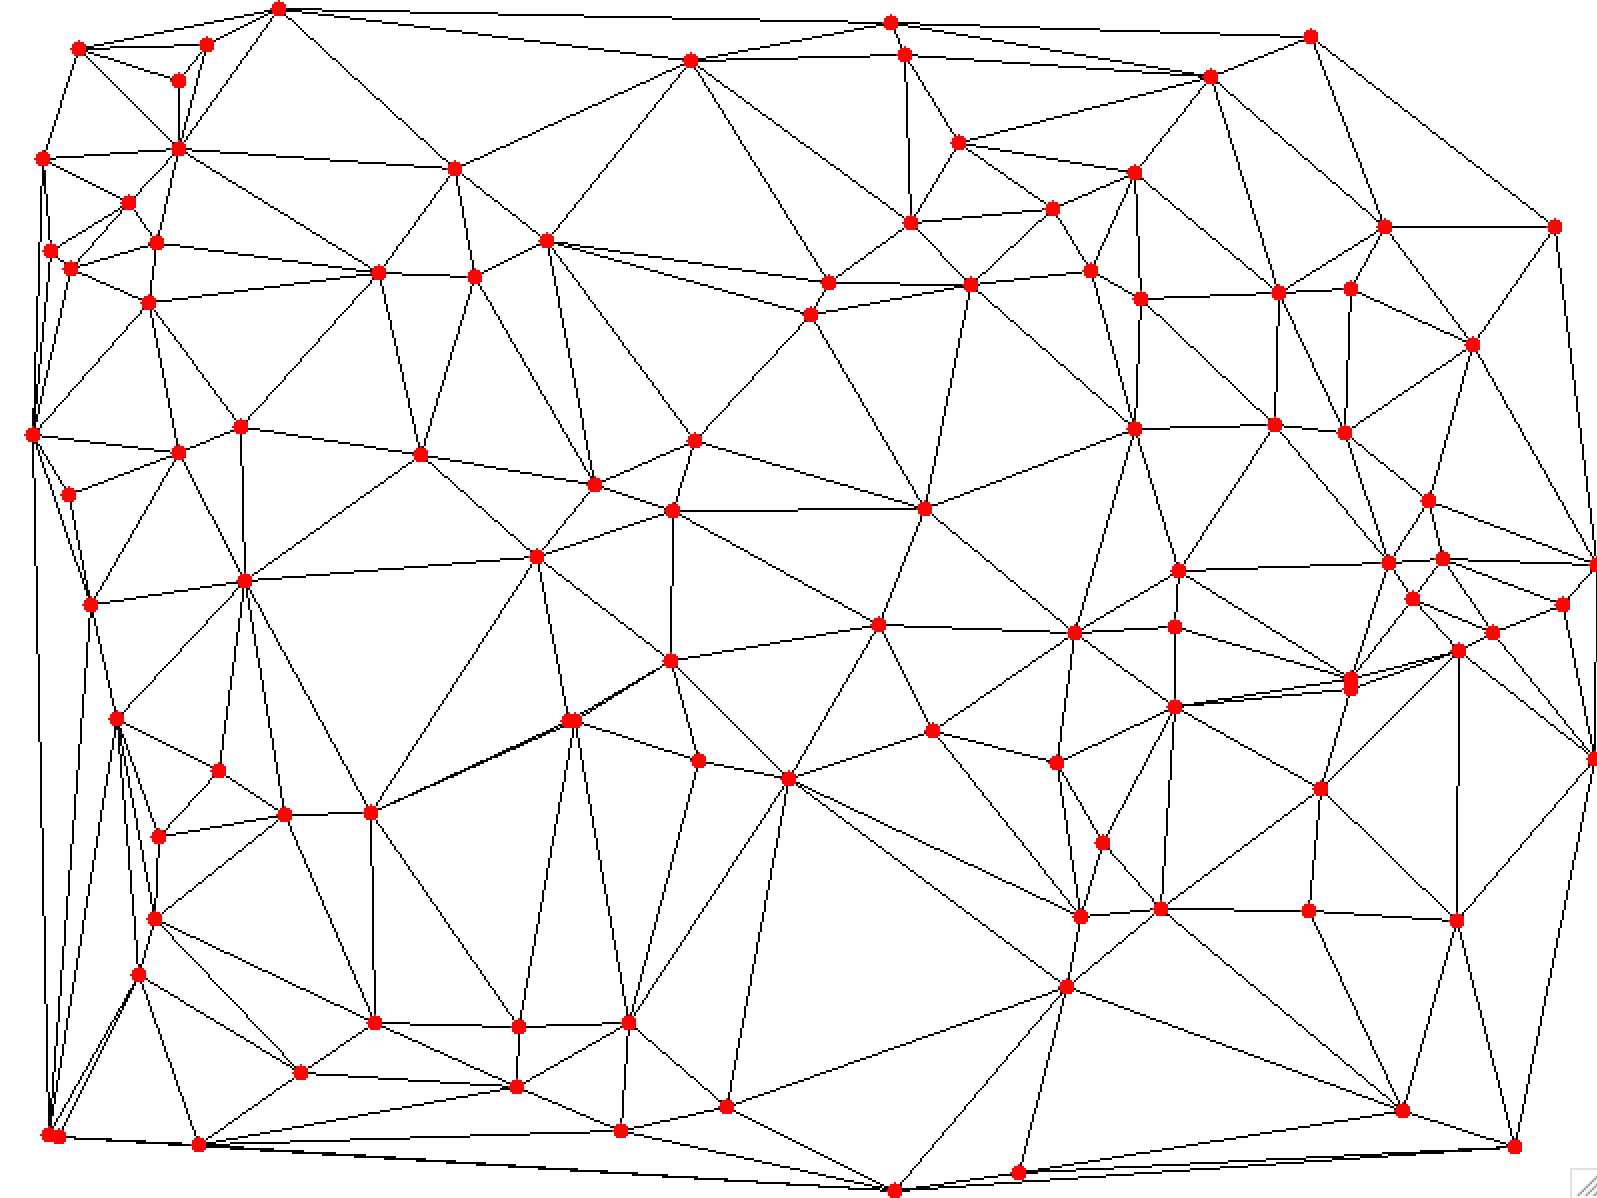
\includegraphics[scale=0.3]{convexhull-good.png}
	\end{center}
	\caption{Delaunay's triangulation starting with convex hull}
	\label{fig:good}
\end{figure}

\subsection{Convex hull}
To start the triangulation I had to compute which points were on the convex hull. I did it using the gift wrapping algorithm. This method is based on comparing angles between segment. The function that compute angle was hard in the way that it required the find the right order to pass segments.

\subsection{Nearly flat triangle}
With the convex hull we have to create the first triangles to then start the triangulation. I tried a few methods : 
\begin{itemize}
	\item adding a point in the middle to then create triangles with an edge of the convex hull and the center points;
	\item cut in half the convex hull recursively and shift each time to avoid that all triangles have a common point. 
\end{itemize}

While these create good looking first generation triangles, it can then mess-up everything during the process of triangulation with edges that cut other ones as seen in the figure~\ref{fig:messedup}.

\begin{figure}[H]
	\centering
	\begin{subfigure}{.5\textwidth}
		\begin{center}
			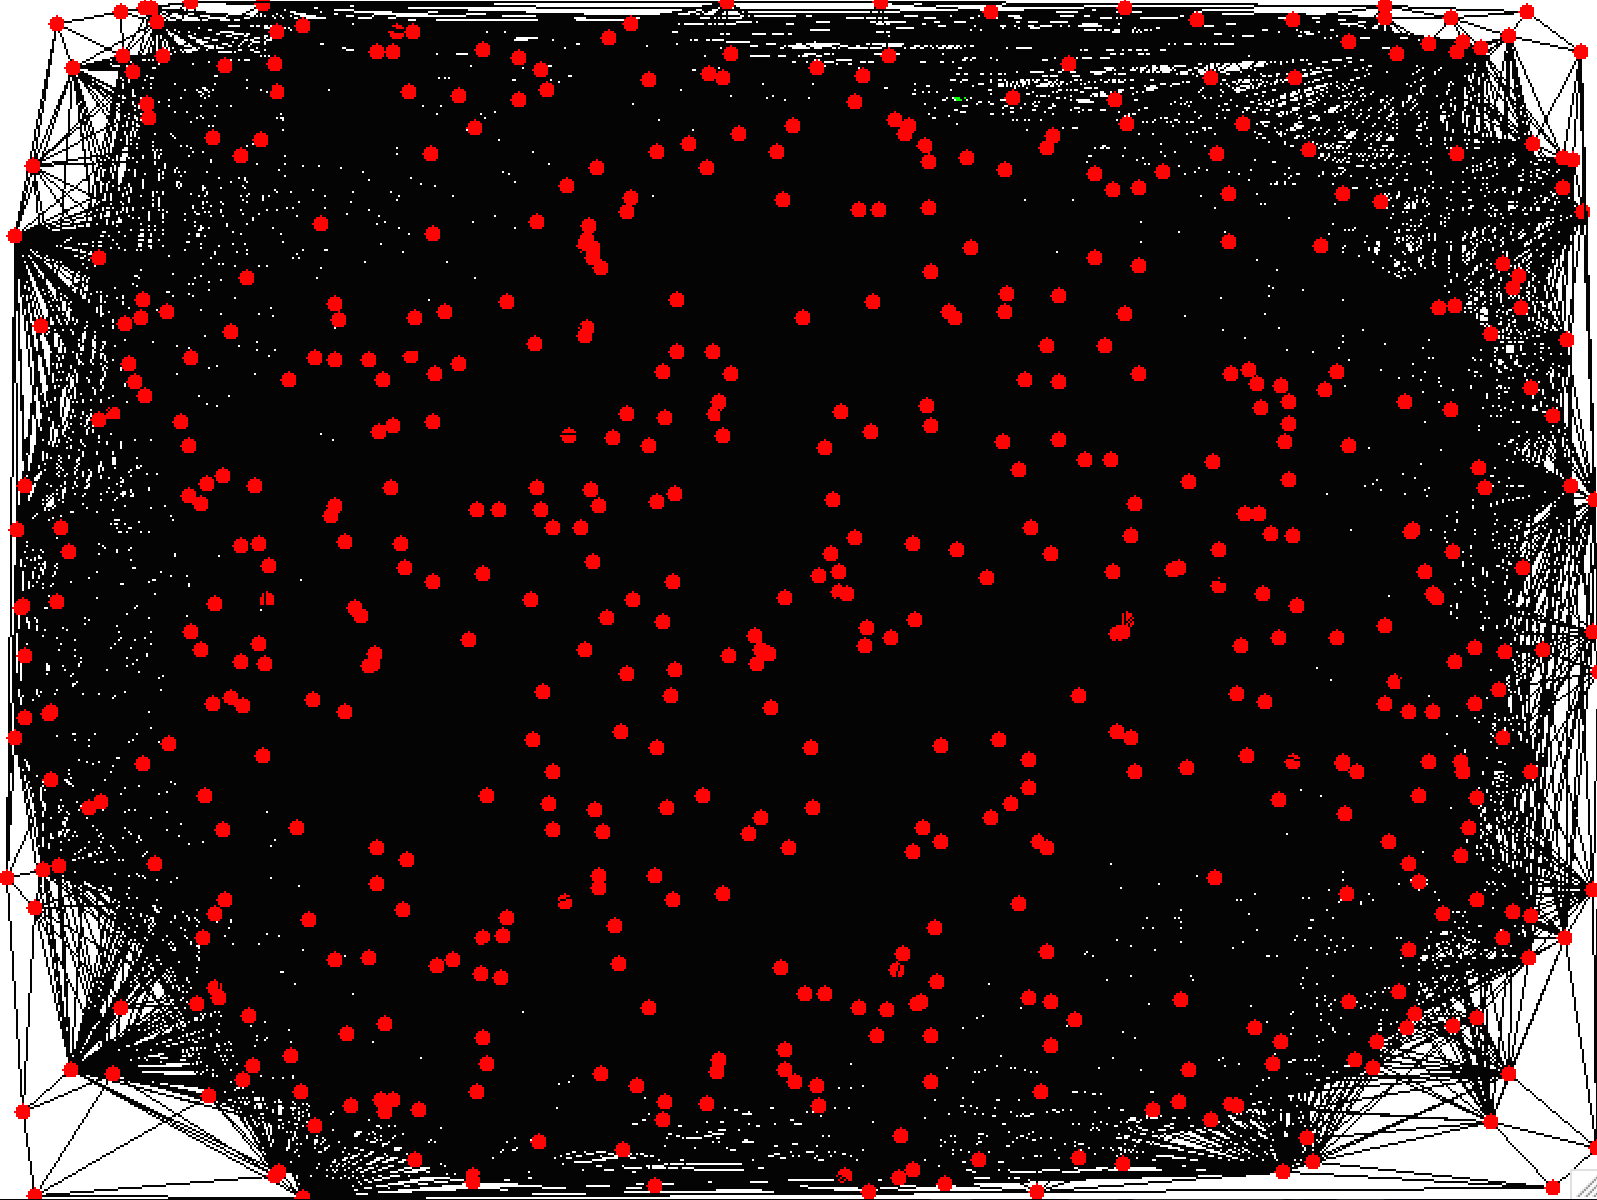
\includegraphics[width=0.99\linewidth]{convexhull-messedup.png}
		\end{center}
		\caption{With 600 points}
		\label{fig:verymessedup}
	\end{subfigure}%
	\begin{subfigure}{.5\textwidth}
		\begin{center}
			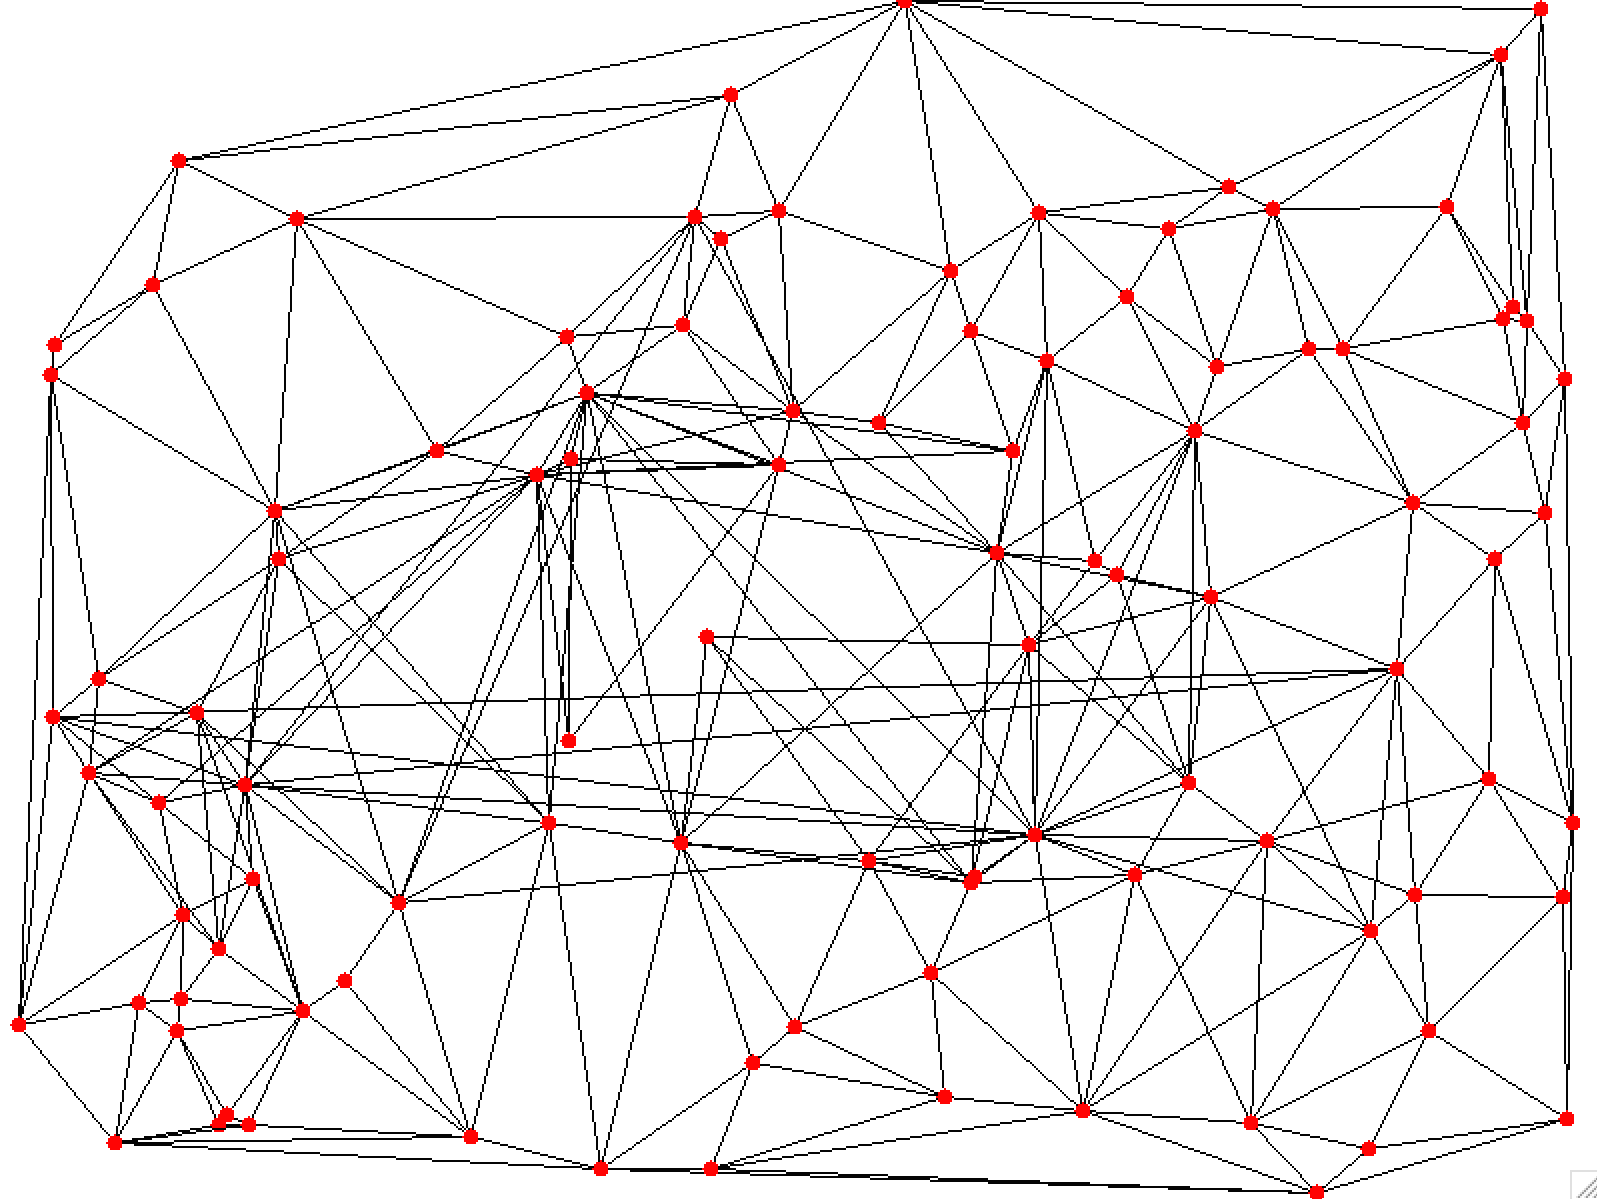
\includegraphics[width=0.99\linewidth]{convexhull-messedup-abit.png}
		\end{center}
		\caption{With 100 points}
		\label{fig:messedupabit}
	\end{subfigure}
	\caption{Bad Delaunay's triangulations}
	\label{fig:messedup}
\end{figure}

This is due to nearly flat triangles that have huge circumscribed circles, which envelop points that are far away. These don't occur when we start with a rectangle because we start with only two big triangles so when we add a new point. Either it's close to the border and so the big circumscribed circle is on the outside,  either all triangles are reshaped and that avoid having a flat new triangle.

\section{Conclusion}
After all, I haven't done much more than the basic version required for the project. Even though I put quite a lot of work in the convex hull part, both on computing the convex hull part and using it, it has not paid.


\clearpage % Pour être sûr que toutes les figures sont bien éjectées

\appendix % Passer en numérotation en lettres


\section{Annex: self evaluation}

\subsubsection*{Strengths}
\begin{itemize}
\item Straight forward approach, easy to understand.
\end{itemize}

\subsubsection*{Weaknesses}
\begin{itemize}
\item Non optimized ;
\item still existing bugs.
\end{itemize}

\subsubsection*{Opportunities}
\begin{itemize}
\item 
\end{itemize}

\subsubsection*{Threats}
\begin{itemize}
\item 
\end{itemize}


\end{document}

